\documentclass[14pt]{extbook}
\usepackage{multicol, enumerate, enumitem, hyperref, color, soul, setspace, parskip, fancyhdr} %General Packages
\usepackage{amssymb, amsthm, amsmath, latexsym, units, mathtools} %Math Packages
\everymath{\displaystyle} %All math in Display Style
% Packages with additional options
\usepackage[headsep=0.5cm,headheight=12pt, left=1 in,right= 1 in,top= 1 in,bottom= 1 in]{geometry}
\usepackage[usenames,dvipsnames]{xcolor}
\usepackage{dashrule}  % Package to use the command below to create lines between items
\newcommand{\litem}[1]{\item#1\hspace*{-1cm}\rule{\textwidth}{0.4pt}}
\pagestyle{fancy}
\lhead{Makeup Progress Quiz 2}
\chead{}
\rhead{Version C}
\lfoot{2790-1423}
\cfoot{}
\rfoot{Summer C 2021}
\begin{document}

\begin{enumerate}
\litem{
Choose the graph of the equation below.\[ f(x) = \frac{-1}{x - 2} - 1 \]\begin{enumerate}[label=\Alph*.]
\begin{multicols}{2}\item 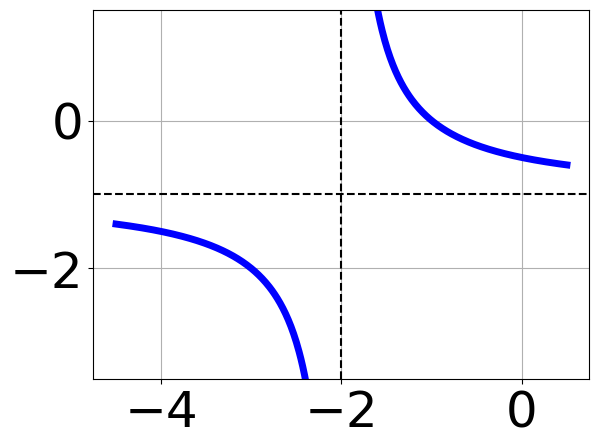
\includegraphics[width = 0.3\textwidth]{../Figures/rationalEquationToGraphAC.png}\item 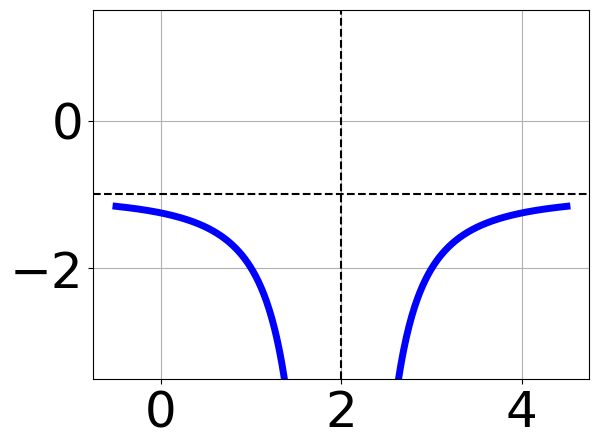
\includegraphics[width = 0.3\textwidth]{../Figures/rationalEquationToGraphBC.png}\item 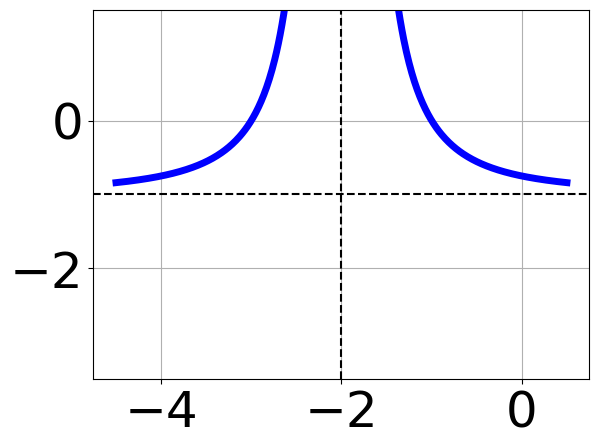
\includegraphics[width = 0.3\textwidth]{../Figures/rationalEquationToGraphCC.png}\item 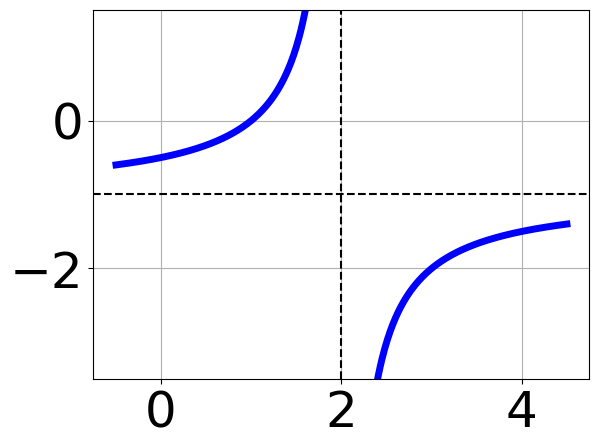
\includegraphics[width = 0.3\textwidth]{../Figures/rationalEquationToGraphDC.png}\end{multicols}\item None of the above.
\end{enumerate} }
\litem{
Solve the rational equation below. Then, choose the interval(s) that the solution(s) belongs to.\[ \frac{7}{3x -8} + 8 = \frac{2}{9x -24} \]\begin{enumerate}[label=\Alph*.]
\item \( \text{All solutions lead to invalid or complex values in the equation.} \)
\item \( x \in [1.4,4.4] \)
\item \( x_1 \in [-3.93, 0.07] \text{ and } x_2 \in [2.4,2.41] \)
\item \( x_1 \in [-0.6, 5.4] \text{ and } x_2 \in [2.41,2.54] \)
\item \( x \in [-3.93,0.07] \)

\end{enumerate} }
\litem{
Choose the graph of the equation below.\[ f(x) = \frac{-1}{(x - 1)^2} + 2 \]\begin{enumerate}[label=\Alph*.]
\begin{multicols}{2}\item 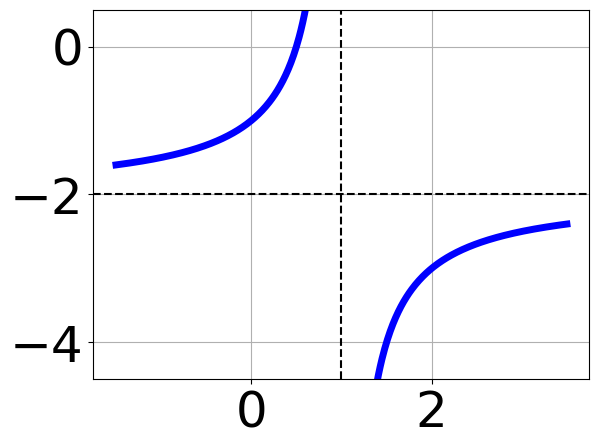
\includegraphics[width = 0.3\textwidth]{../Figures/rationalEquationToGraphCopyAC.png}\item 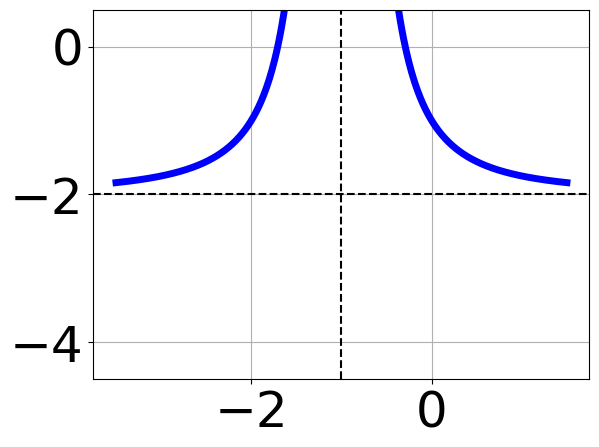
\includegraphics[width = 0.3\textwidth]{../Figures/rationalEquationToGraphCopyBC.png}\item 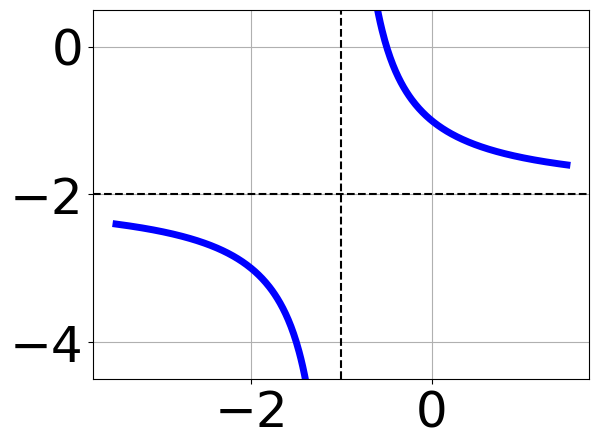
\includegraphics[width = 0.3\textwidth]{../Figures/rationalEquationToGraphCopyCC.png}\item 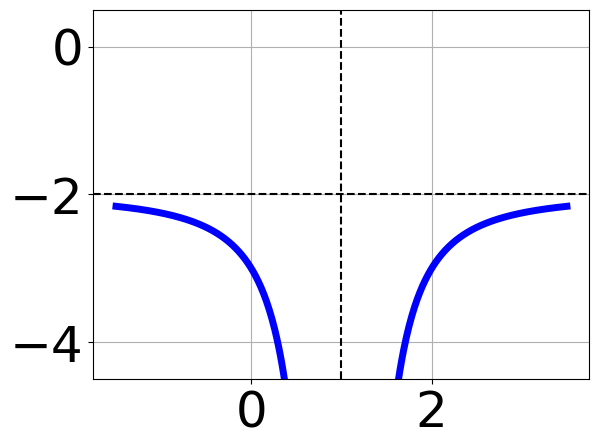
\includegraphics[width = 0.3\textwidth]{../Figures/rationalEquationToGraphCopyDC.png}\end{multicols}\item None of the above.
\end{enumerate} }
\litem{
Solve the rational equation below. Then, choose the interval(s) that the solution(s) belongs to.\[ \frac{-8}{6x -3} + -5 = \frac{-7}{-36x + 18} \]\begin{enumerate}[label=\Alph*.]
\item \( x \in [-1.2,-0.4] \)
\item \( x_1 \in [-0.7, 1.1] \text{ and } x_2 \in [0.3,0.7] \)
\item \( x \in [0.19,4.19] \)
\item \( \text{All solutions lead to invalid or complex values in the equation.} \)
\item \( x_1 \in [-1.2, -0.4] \text{ and } x_2 \in [-0.7,0.3] \)

\end{enumerate} }
\litem{
Determine the domain of the function below.\[ f(x) = \frac{5}{24x^{2} +6 x -9} \]\begin{enumerate}[label=\Alph*.]
\item \( \text{All Real numbers.} \)
\item \( \text{All Real numbers except } x = a \text{ and } x = b, \text{ where } a \in [-13, -10] \text{ and } b \in [17, 21] \)
\item \( \text{All Real numbers except } x = a, \text{ where } a \in [-0.75, 0.25] \)
\item \( \text{All Real numbers except } x = a \text{ and } x = b, \text{ where } a \in [-0.75, 0.25] \text{ and } b \in [0.5, 3.5] \)
\item \( \text{All Real numbers except } x = a, \text{ where } a \in [-13, -10] \)

\end{enumerate} }
\litem{
Choose the equation of the function graphed below.
\begin{center}
    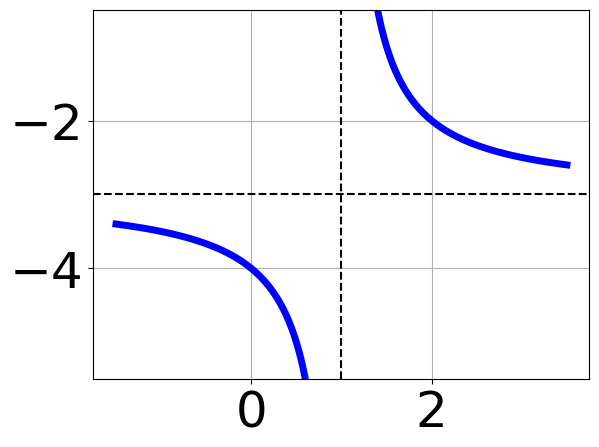
\includegraphics[width=0.5\textwidth]{../Figures/rationalGraphToEquationC.png}
\end{center}
\begin{enumerate}[label=\Alph*.]
\item \( f(x) = \frac{1}{x - 1} - 4 \)
\item \( f(x) = \frac{1}{(x - 1)^2} - 4 \)
\item \( f(x) = \frac{-1}{x + 1} - 4 \)
\item \( f(x) = \frac{-1}{(x + 1)^2} - 4 \)
\item \( \text{None of the above} \)

\end{enumerate} }
\litem{
Determine the domain of the function below.\[ f(x) = \frac{3}{20x^{2} +x -30} \]\begin{enumerate}[label=\Alph*.]
\item \( \text{All Real numbers except } x = a \text{ and } x = b, \text{ where } a \in [-21, -18] \text{ and } b \in [28, 34] \)
\item \( \text{All Real numbers except } x = a, \text{ where } a \in [-2.25, 0.75] \)
\item \( \text{All Real numbers except } x = a, \text{ where } a \in [-21, -18] \)
\item \( \text{All Real numbers except } x = a \text{ and } x = b, \text{ where } a \in [-2.25, 0.75] \text{ and } b \in [-0.8, 3.2] \)
\item \( \text{All Real numbers.} \)

\end{enumerate} }
\litem{
Choose the equation of the function graphed below.
\begin{center}
    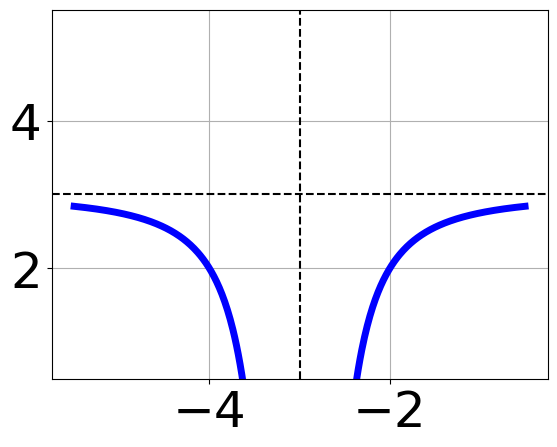
\includegraphics[width=0.5\textwidth]{../Figures/rationalGraphToEquationCopyC.png}
\end{center}
\begin{enumerate}[label=\Alph*.]
\item \( f(x) = \frac{1}{x - 3} + 3 \)
\item \( f(x) = \frac{-1}{(x + 3)^2} + 3 \)
\item \( f(x) = \frac{1}{(x - 3)^2} + 3 \)
\item \( f(x) = \frac{-1}{x + 3} + 3 \)
\item \( \text{None of the above} \)

\end{enumerate} }
\litem{
Solve the rational equation below. Then, choose the interval(s) that the solution(s) belongs to.\[ \frac{3x}{-5x + 5} + \frac{-2x^{2}}{-35x^{2} +10 x + 25} = \frac{-2}{7x + 5} \]\begin{enumerate}[label=\Alph*.]
\item \( x_1 \in [-0.76, -0.74] \text{ and } x_2 \in [-0.29,1.06] \)
\item \( x \in [-0.74,-0.67] \)
\item \( x \in [0.96,1] \)
\item \( \text{All solutions lead to invalid or complex values in the equation.} \)
\item \( x_1 \in [0.96, 1] \text{ and } x_2 \in [-1.5,-0.63] \)

\end{enumerate} }
\litem{
Solve the rational equation below. Then, choose the interval(s) that the solution(s) belongs to.\[ \frac{6x}{-6x -2} + \frac{-5x^{2}}{-18x^{2} +6 x + 4} = \frac{4}{3x -2} \]\begin{enumerate}[label=\Alph*.]
\item \( x \in [-0.69,-0.24] \)
\item \( x_1 \in [-1.03, -0.38] \text{ and } x_2 \in [0.01,0.36] \)
\item \( x_1 \in [-0.69, -0.24] \text{ and } x_2 \in [0.59,0.96] \)
\item \( x \in [0.6,1.75] \)
\item \( \text{All solutions lead to invalid or complex values in the equation.} \)

\end{enumerate} }
\end{enumerate}

\end{document}